% generated by plots/fig3_wealth.py --- do not edit the numbers by hand
% figure* --- the chapter is two-column and this does not fit one
\begin{figure*}[tp]
\centering
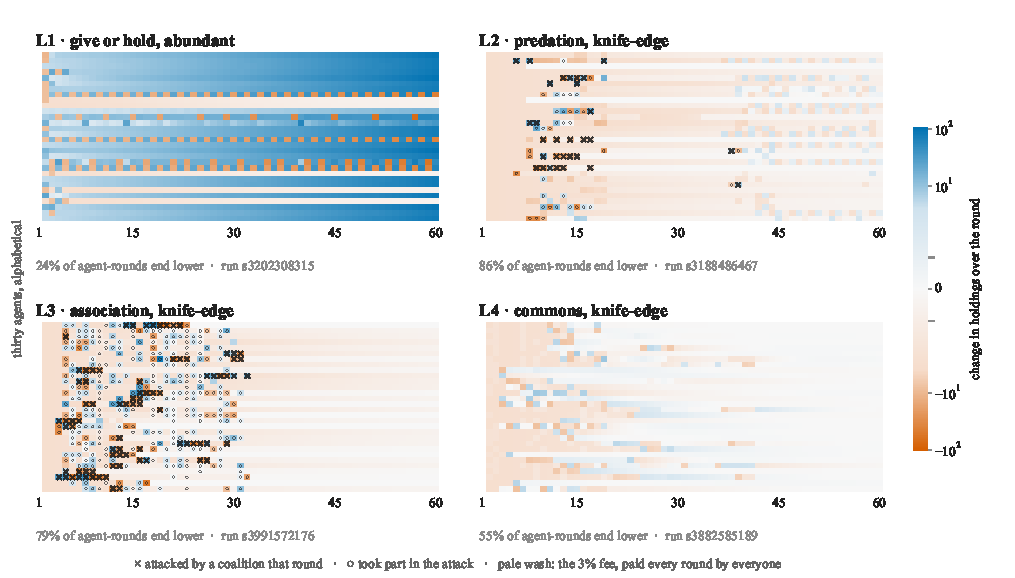
\includegraphics[width=\linewidth]{figures/fig3_wealth/deltas.pdf}\\[2pt]
\caption[What each round does to what an agent holds]{%
\textbf{What each round does to what an agent holds.} Thirty agents down the side in alphabetical order, sixty rounds across, and a cell coloured by the change over that round, blue for a gain and vermilion for a loss and pale where little happened. A cross marks the agent a coalition attacked that round and an open dot each agent that joined it, which is what separates a loss to a blow from the slow bleed of the fee. The scale is symmetric and logarithmic either side of zero, since the median round is a loss of one resource and the worst a loss of a hundred. One run per capacity level, each the run whose final inequality is its cell's median: \texttt{s3202308315} (L1 abundant, 24\% of agent-rounds ending lower); \texttt{s3188486467} (L2 knife-edge, 86\% of agent-rounds ending lower); \texttt{s3991572176} (L3 knife-edge, 79\% of agent-rounds ending lower); \texttt{s3882585189} (L4 knife-edge, 55\% of agent-rounds ending lower).}
\label{fig:wealth}
\end{figure*}
